\begin{figure}[ht]
	\centering
	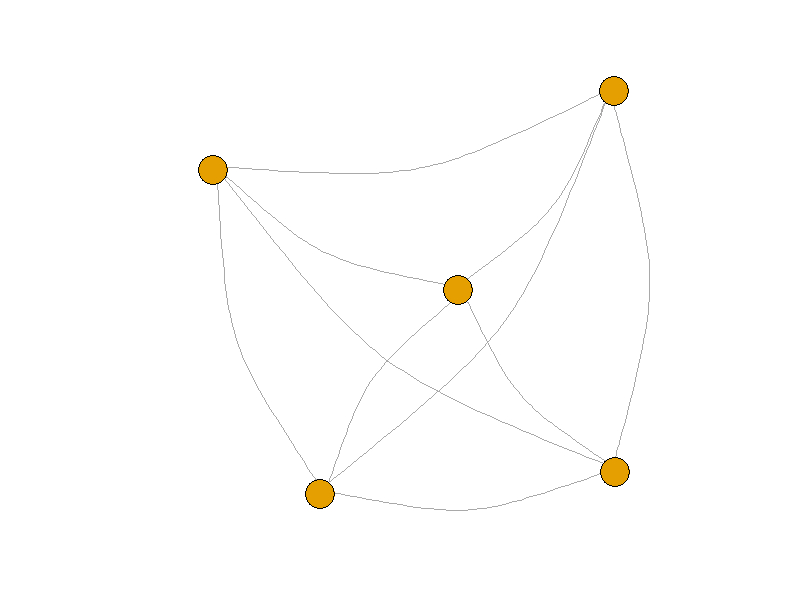
\includegraphics[height=6cm]{partials/images/graph_full.png}
	\caption{Przykładowy wygenerowany graf pełny}
	\label{Fig:tests-generation-1}
\end{figure}
\FloatBarrier

Dane wygenerowane zostały przy pomocy skryptu stworzonego w języku R oraz biblioteki igraph.
Skrypt został zaprojektowany funkcyjnie, by osiągnąć możliwie największą automatyzację testów.
Rysunki grafów tworzone są o wielkości 800x600 pikseli, na białym tle, z wierzchołkami w kolorze pomarańczowym,
bez jakichkolwiek oznaczeń wierzchołków oraz zapisywane są w odpowiednich katalogach, odpowiadających klasie grafu.
Przygotowane zostały funkcje tworzące ścieżki, cykle, grafy pełne, grafy bezkrawędziowe oraz drzewa binarne.
W każdej z funkcji możliwy jest wybór liczby generowanych grafów, liczba wierzchołków grafu
oraz współczynnik odpowiadający za zakrzywienie krawędzi na rysunkach.

\begin{lstlisting}[language=R,caption=Listing skryptu rysującego grafy,label={tests-generation-1}]
	#' Rysuj graf
	#'
	#' @param graph Graph - Graf do narysowania
	#' @param pathName string - Sciezka
	#' @param fileName string - Nazwa pliku
	#' @param vertexNo int - liczba wierzcholkow
	#' @param i int - Numer iteracji
	#' @param plotCurve float
	#' @return void
	#'
	plotGraphHelper <- function(graph, pathName, fileName, vertexNo, i, plotCurve)
	{
	  png(file.path(pathName, paste0(fileName, "-", vertexNo, "-", i, ".png")), width = 800, height = 600)
	  plot(graph, vertex.label = NA, edge.curved = plotCurve)
	  dev.off()
	}
\end{lstlisting}

\begin{lstlisting}[language=R,caption=Listing funkcji tworzącej ścieżkę,label={tests-generation-2}]
	#' Graf sciezka N wierzcholkow, nieskierowany
	#'
	#' @param N int - liczba rysunkow
	#' @param vertexNo int - liczba wierzcholkow
	#' @param plotCurve float
	#' @return void
	#'
	plotPaths <- function(N, vertexNo, plotCurve)
	{
		fileName <- 'path'
		pathName <- createDir(vertexNo, fileName)
		definition <- c()
		for (index in 1:(vertexNo-1))
		{
			definition <- c(definition, index, index + 1)
		}
		definitionMatrix <- matrix(definition, ncol = 2, byrow = TRUE)
		
		for (i in 1:N)
		{
			graph <- graph_from_edgelist(definitionMatrix, directed = FALSE)
			E(graph)$weight <- runif(ecount(graph))
			plotGraphHelper(graph, pathName, fileName, vertexNo, i, plotCurve)
		}
	}
\end{lstlisting}

W testach wykorzystane zostały wszystkie wybrane typy grafów.
Każdy z nich, czyli dana liczba wierzchołków i typ grafu, wygenerowany został w liczbie 500 sztuk
oraz ze stałą krzywizną krawędzi, wynoszącą 0,3.